%%%%%%%%%%%%%%%%%%%%%
% !TeX spellcheck = en_GB
\section{Saturday, \SI{24}{\dec}}\label{sec:2412}

%%% short info on Saturdays general weather
\SI{24}{\dec} was characterised by moderate precipitation with a total \SI{24}{\hour} accumulation of \SI{24}{\mm}. In the beginning of the day was the temperature close to zero and then dropped to a minimum of \SI{- 5}{\celsius} in the afternoon. On this day, the centre of the low pressure system, was lying between Iceland and North-West Norway with a continuous wind from the west, which became stronger towards the evening.

%%%%%%%%%%%%%%%%%%%%%%%%%%%%%%%%%%%%%%%%%%%%%%%%%%%%%%%%%%%%%%%%%%%%%%%%%%
%%%%%%%%% surface obs %%%%%%%%%%%%%%
\subsection{Surface accumulation}\label{sec:2412:surface}
As discussed early seems the surface precipitation amount on \SI{24}{\dec} not to be influenced by too little precipitation which \cite{muller_arome-metcoop:_2017} showed to be the case for precipitation amount up to \SI{10}{\mm}. 
%%% image surface MEPS boxplot %%%%%%%%%%%%%%%%%%%%%%%%%%%%%%%%%%%%%
\begin{figure}[t]
	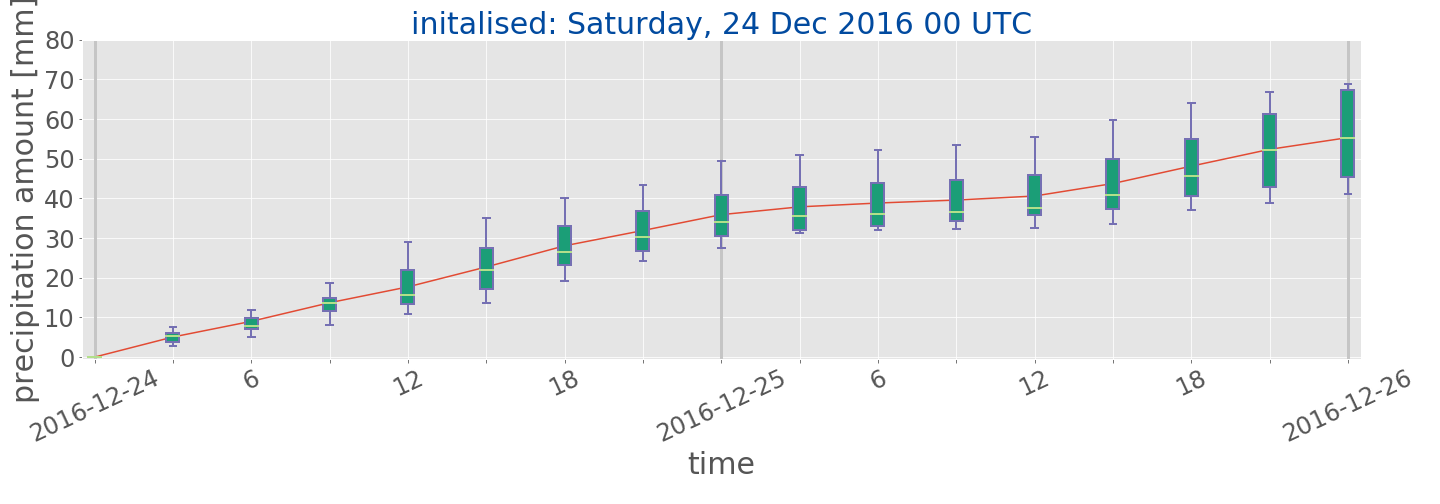
\includegraphics[width=\textwidth]{./fig_boxplot_sfc/20161224_0}
	\caption{Box-whisker-plot of the ten ensemble members of MEPS. Red line indicating the ensemble mean, lower and upper whisker the 25th and 75th percentile, respectively. Light green shows the median of all members and the box represents the middle \SI{50}{\percent} of scores of the precipitation.}\label{fig:boxplt24}
\end{figure}
%%%%%%%%%%%%%%%%%%%%%%%%%%%%%%%%%%%%%%%%%%%%%%%%%%%%%%%%%%%%%%%%%%%%%%%%%%
To understand what might have led to the overestimation of surface precipitation on the \SI{24}{\dec} in \Cref{fig:sfc_acc24}, a box-whisker-plot is presented. Compared to \SI{21}{\dec} shows the box-whisker-plot in \Cref{fig:boxplt24} an uncertainty between the ten ensemble members already after \SI{3}{\hour} forecast time. The spread between the ensemble members (shown by the minimum and maximum whiskers) seems to be wide. Not all ten members agree on the same precipitation amount as they did for example on \SI{21}{\dec}.
\\
The ensemble mean (red line) is always higher than the median and already after \SI{12}{\hour} forecast time is the median closer to the lower 25th percentile. Also, all upper whiskers are taller than the lower ones, which would follow that the ensemble members vary amongst the most positive quartile and that it is very similar for the least positive quartile group.
A comparison with \Cref{fig:sfc_acc24} shows that most of the member lie beneath the ensemble mean (dashed, blue line). On \SI{24}{\dec} the ensemble mean is much lower than the deterministic forecast, which lies closer to the 50th percentile. This is not for all days the case, on most of the days is the ensemble mean either similar or a little less to the deterministic forecast. Since the deterministic forecast, black line in \Cref{fig:sfc_acc24}, is in the upper percentile compared to its perturbed members it follows that for this forecast the deterministic forecast was not the best guess for the surface accumulation and by using the 'wrong' initial state it can have led to larger miscalculations. Therefore, it would be interesting to perform a new deterministic forecast and its associated perturbations to see if a change in choosing another initial state results in a similar measured precipitation amount at the ground.
\\
\\
The uncertainty appearing already after \SI{3}{\hour} can be associated with a too long spin-up time of MEPS. To represent the surface accumulation well, the model systems needs to be spin-up. The regional model MEPS needs initial and boundary conditions from ECMWF before it can produce forecasts. Since initial conditions such as observations have uncertainties as well as the model has mistrust and needs to approach its own climatology, a model has to stabilize before the simulations can be trusted. The spin-up time varies depending on the quality of the initial and boundary conditions. Apparently, it seems, that the initial and boundary conditions for MEPS were not perfect on \SI{24}{\dec} at \SI{0}{\UTC} since the deterministic and perturbed members seem not to have stabilised yet and show uncertainties in \Cref{fig:boxplt24} from early on.  At this point it might be interesting to re-run the initialisation again with all available observations to see, if that might have an influence on the overestimation observed in \Cref{fig:sfc_acc24}. It might not necessarily be the observations. Since, ECMWF is the boundary condition of MEPS it could also be that the ECMWF forecast did not have reached its stabilised state when MEPS was initiated.
\\
The uncertainty might also have resulted from the fact, that the precipitation around \SI{0}{\UTC} on \SI{24}{\dec} was higher than on the previous days (see, \Cref{fig:TPU}). Where on the previous days the hourly precipitation around \SI{0}{\UTC} was less intense might a big accretion have followed an uncertainty already after \SI{3}{\hour}. MEPS initialised on \SI{24}{\dec} at \SI{0}{\UTC} might have accounted for an additional precipitation at \SI{12}{\UTC} on \SI{24}{\dec} and that led to the strong increase at \SI{13}{\UTC}. This might be a local effect, that a precipitation cell in the model was spatially misplaced or a by a few kilometres or a higher precipitation amount was expected by the model and actually did not occur at Haukeliseter rather at another site close to Haukeliseter, and followed that strong increase after noon. 
\\
It is therefore important as the double fence construction or measurements from the MRR to give models a good initial condition from observations, so that spin-up time can be reduced and model initialisation start at a realistic state.


% %%%%%%%%%%%%%%%%%%%%%%%%%%%%%%%%%%%%%%%%%%%%%%%%%%%%%%%%%%%%%%%%%%%%%%%%%%
% %%%%%%%%% vertical obs %%%%%%%%%%%%%%
% \subsection{Vertical snowfall observations}\label{sec:vertEM09:2412}
% % %%% image SWP %%%%%%%%%%%%%%%%%%%%%%%%%%%%%%%%%%%%%
% \begin{figure}[t]
% 	\centering
% 	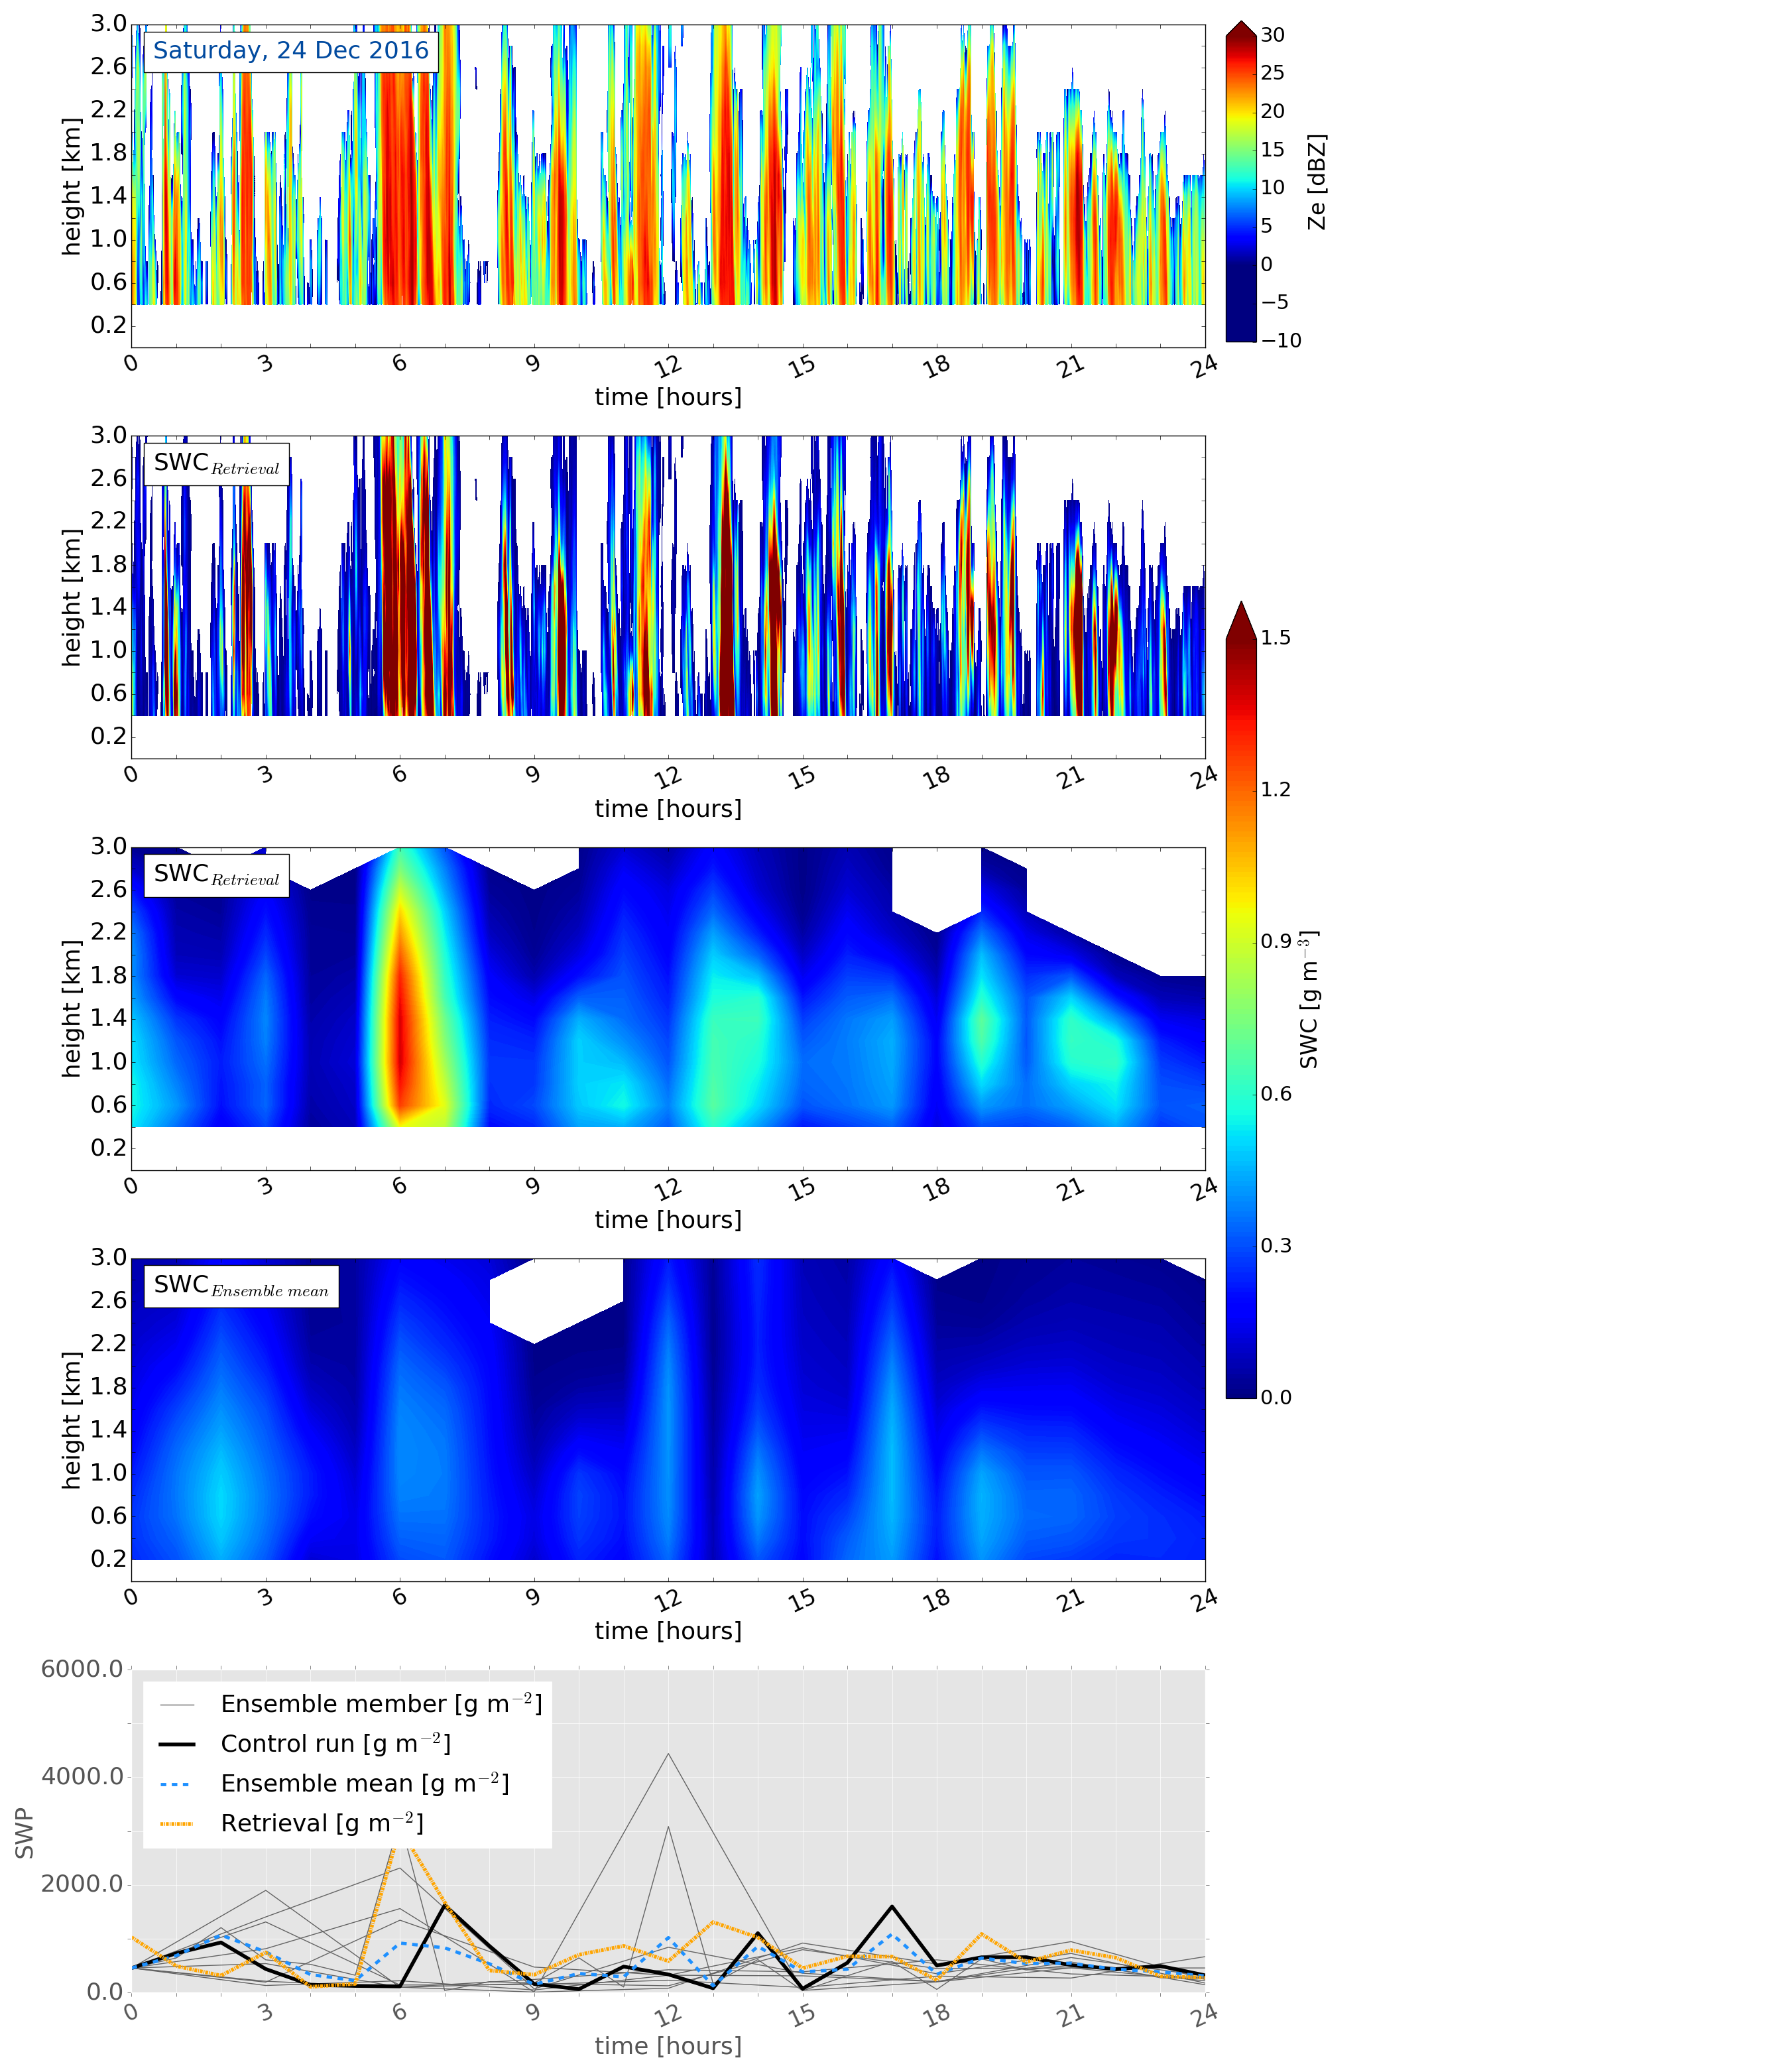
\includegraphics[trim={0.4cm .4cm 31.3cm 63.5cm},clip,width=\textwidth]{./fig_SWC/20161224}
% 	\caption{}\label{fig:SWP24}
% \end{figure}
% %%%%%%%%%%%%%%%%%%%%%%%%%%%%%%%%%%%%%%%%%%%%%%%%%%%%%%%%%%%%%%%%%%%%%%%%%%
% % text
% %
% % %%% image ensemble member 0-9 %%%%%%%%%%%%%%%%%%%%%%%%%%%%%%%%%%%%%
% \begin{figure}[t]
% 	\centering
% 	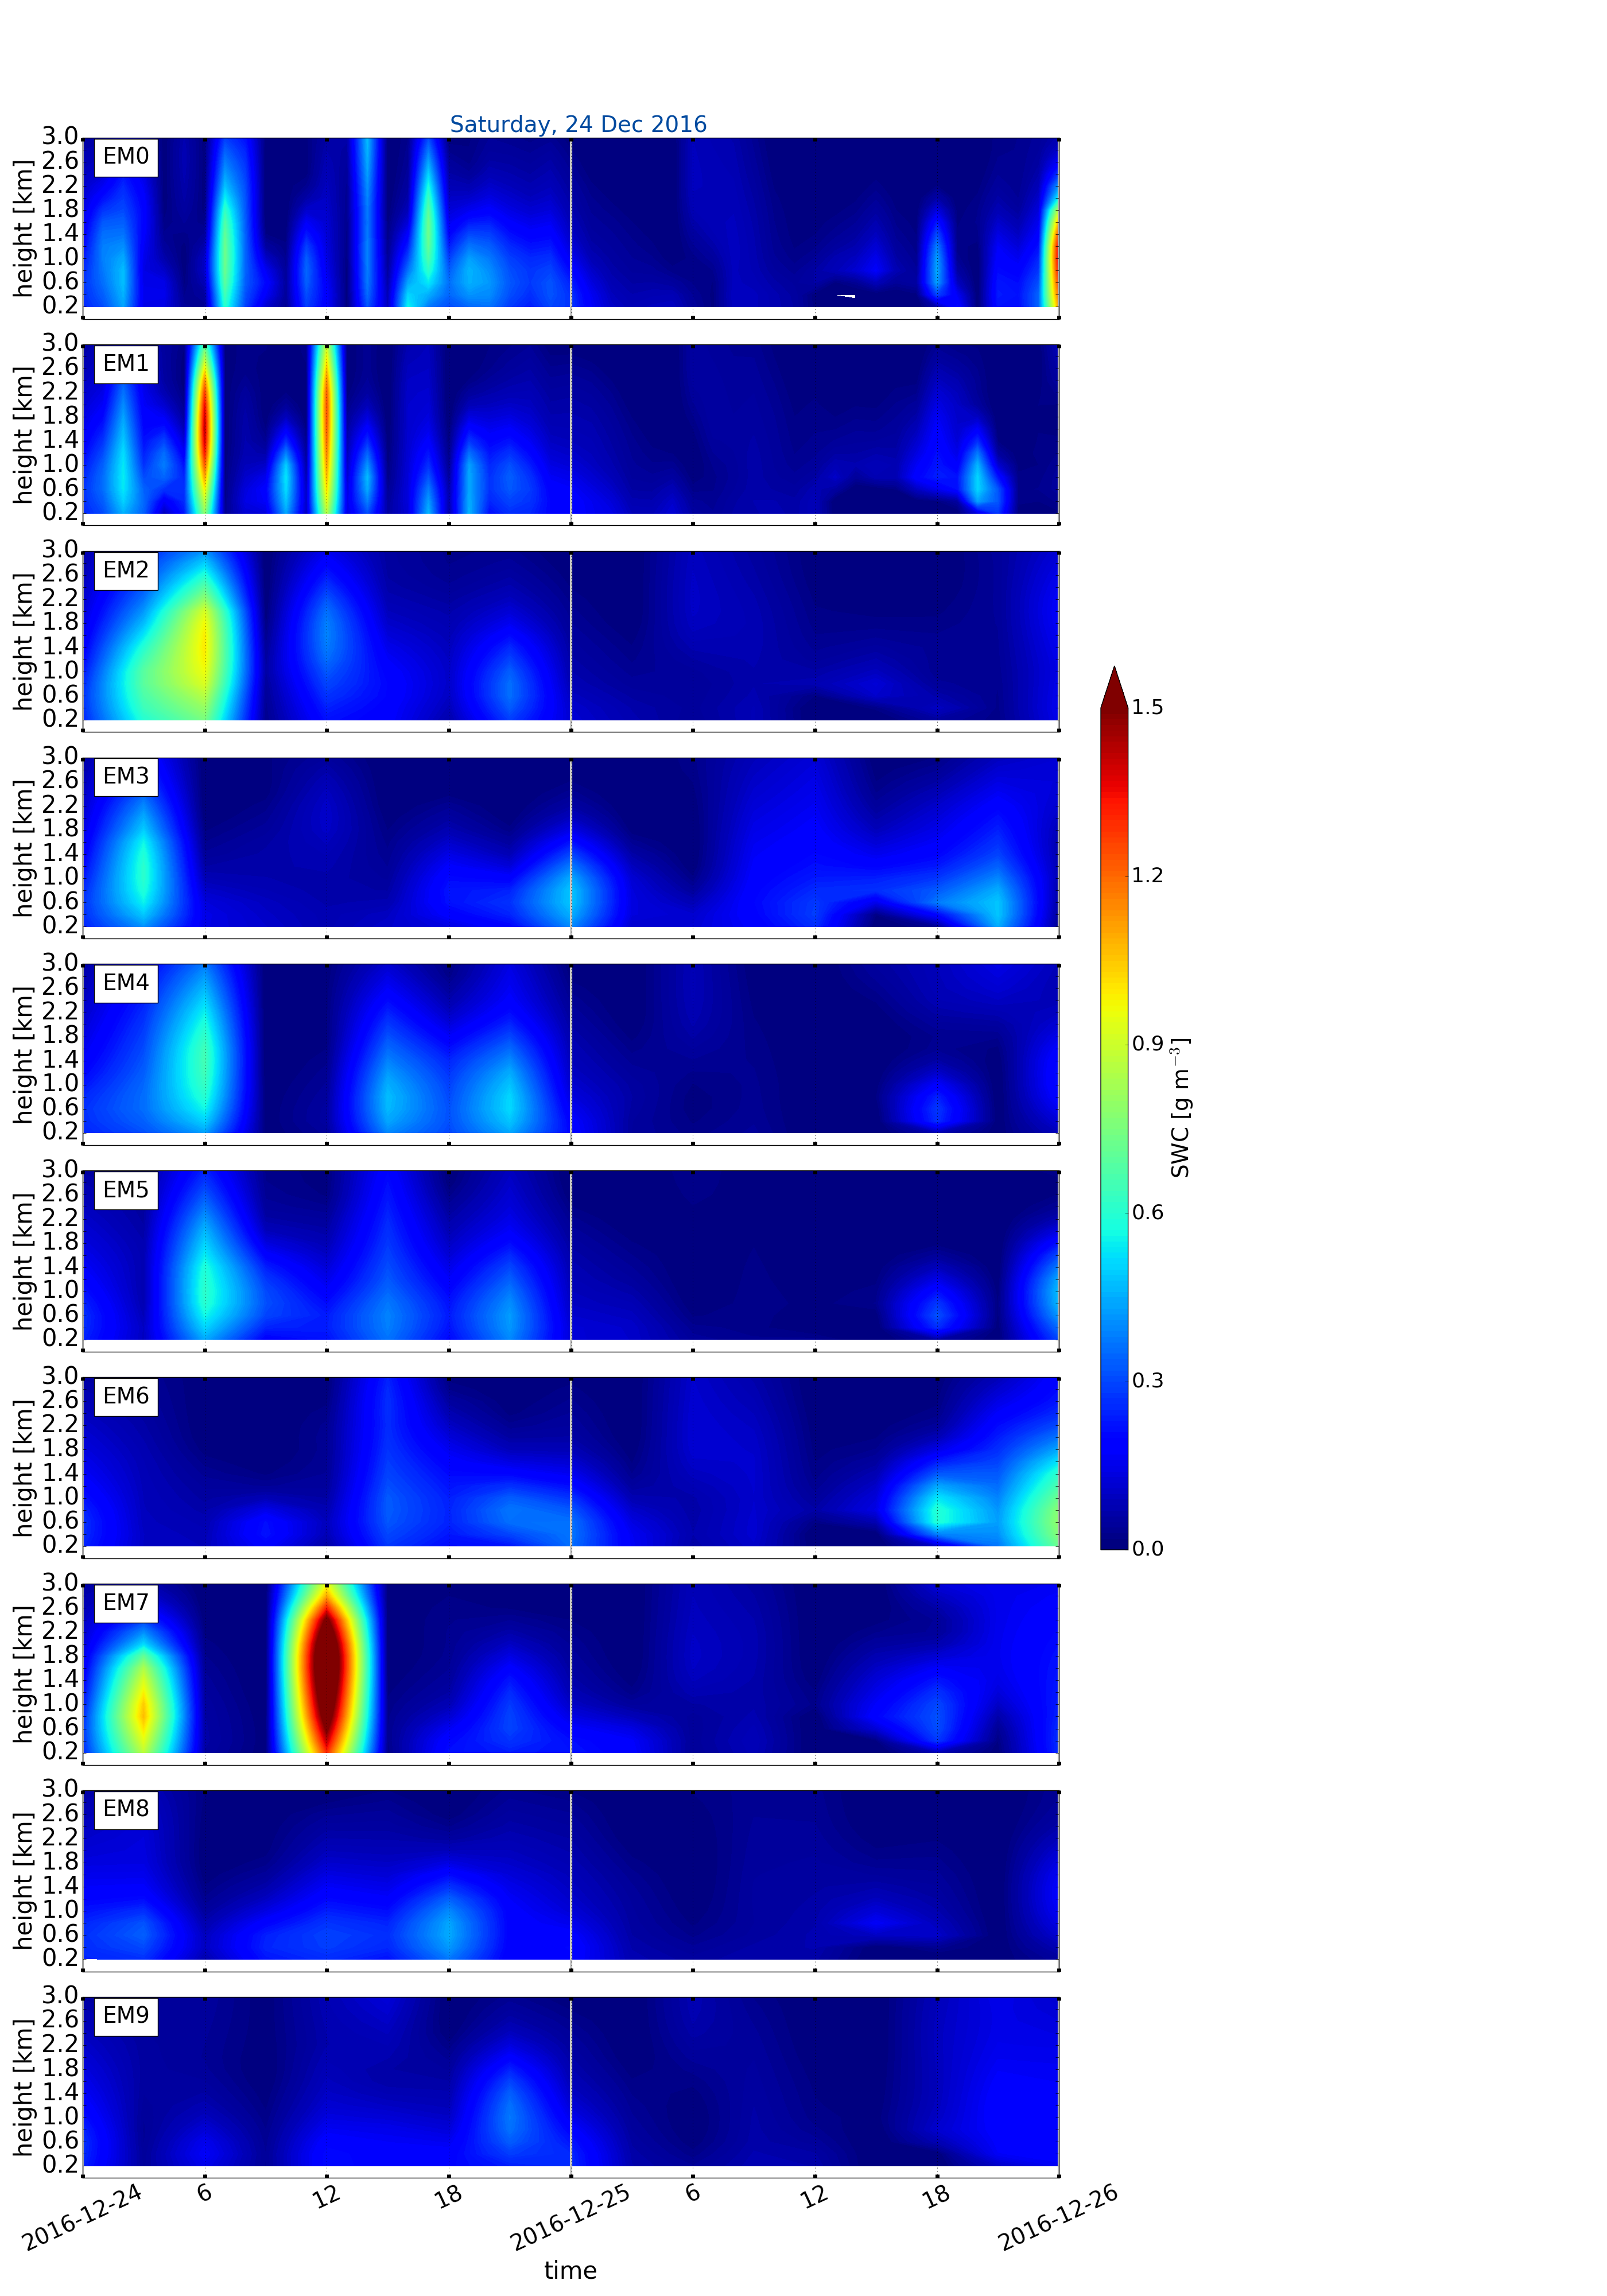
\includegraphics[trim={0cm 0cm 18.3cm 5.1cm},clip,width=0.8\textwidth]{./fig_09EM/20161224}
% 	\caption{SWC of all ensemble members initialised Saturday, \SI{24}{\dec} at 0\SI{0}{\UTC} forecast for \SI{48}{\hour}.}\label{fig:EM09_24}
% \end{figure}
% %%%%%%%%%%%%%%%%%%%%%%%%%%%%%%%%%%%%%%%%%%%%%%%%%%%%%%%%%%%%%%%%%%%%%%%%%%
% \textcolor{red}{DISCUSSION! Bring all into relation and include the verification plots}
